\documentclass[12pt]{report}
\usepackage[top=2.3cm, bottom=2.3cm, left=2.3cm, right=2.3cm, centering]{geometry}
\linespread{1.4}
\usepackage[italian]{babel}
\usepackage[utf8]{inputenc} 
\usepackage{scrlayer-scrpage} 
\ifoot[]{}
\cfoot[]{}
\ofoot[\pagemark]{\pagemark}
\pagestyle{scrplain}
\usepackage[table,xcdraw]{xcolor}
\usepackage{dirtytalk}
\usepackage{subfig}
\usepackage{mathptmx}
\usepackage{titling}
\usepackage{graphicx} 
\usepackage{csquotes}
\usepackage{pdfpages} 
\usepackage[bibstyle=apa, style=apa, citestyle = apa, doi = false, isbn = false, url = false]{biblatex}
\usepackage{hyperref,url}
\setlength\bibitemsep{0.3\itemsep}
\addbibresource{bibliography.bib}
\appto{\bibsetup}{\raggedright}
\usepackage{hyperref}
\usepackage{titlesec} 
\usepackage{float}
\titleformat{\chapter}[block]
  {\normalfont\LARGE\bfseries}{\thechapter.}{0.2em}{\LARGE}
\titlespacing*{\chapter}{0pt}{-18pt}{15pt}
\addbibresource{bibliography.bib}


\begin{document}
%
\includepdf[pages={1}]{frontespizio.pdf}
\begin{titlepage}
 \newcommand{\HRule}{\rule{\linewidth}{0.5mm}}
    \begin{figure}
        \centering
\includegraphics[width = 0.6\textwidth]{img/logo_unipi.png}
    \end{figure}
    \begin{center}
        \textsc{\LARGE{ Laurea Magistrale \\ Informatica Umanistica \\}} 
        \vspace{0.5cm}
        \textsc{\LARGE{ seminario di cultura digitale a.a. 2020/21 \\}}
        \vspace{1cm}
        \Large{
        \textbf{Quando la tecnologia non aiuta: \\ Il caso \textit{App Immuni}\\}}

        \vspace{0.5cm}
        
        {\large{\textit{Alice Isola} (Matr. 545007)\\ }}
        \vspace{0.5cm}
    
    {\bf Sommario}\\
    \end{center}
    \HRule\\
    \textit{Perché un’applicazione così utile come l’app Immuni si è rivelata un totale fallimento?} In questa relazione cercheremo di identificare i problemi legati a Immuni, attraverso l'analisi i temi, le opinioni e i sentimenti più diffusi tra gli utenti su Twitter, utilizzando tecniche di \textit{Natural Language Processing} e  cercando di capire se questi problemi siano solo di natura tecnologica oppure coinvolgono anche aspetti di natura sociale e/o politica.\\
    \HRule
    
\end{titlepage}

\tableofcontents
\thispagestyle{empty}
\clearpage
\setcounter{page}{1}
\addtocontents{toc}{\protect\thispagestyle{empty}}
\addcontentsline{toc}{chapter}{Introduzione}
\input{introduzione.tex}

\chapter{Creazione del corpus e \textit{preprocessesing} dei dati}
Per analizzare al meglio le opinioni dei cittadini sul funzionamento dell'App Immuni si è scelto di soffermarci su ciò che essi scrivevano su Twitter, un social network molto popolare e utilizzato per esprimere in maniera semplice ed immediata opinioni riguardo ad una particolare tematica.

La scelta di utilizzare Twitter come strumento per la raccolta dei dati è giustificata anche da altri due fattori: innanzitutto, dal fatto che, rispetto ad altri social networks come Facebook e Instagram, Twitter è quello con la minore percentuale di profili privati, e in secondo luogo, dalla disponibilità di maggiori strumenti per la raccolta dei dati su questa piattaforma.

\section{La raccolta dei tweet utilizzando la libreria di \textit{scraping Twint}}
Si è scelto quindi di raccogliere i tweet scritti sul tema App Immuni durante un periodo temporale di un anno e mezzo, dal \textbf{1 giugno 2020}, mese in cui il Governo italiano ha rilasciato l'applicazione, fino alla fine dell'anno successivo (31 dicembre 2021). 
Per eseguire questa raccolta si è scelto di utilizzare una libreria di \textit{scraping} per la raccolta di tweet, la libreria \textit{Twint}\footnote{le cui informazioni sono reperibili all'interno del seguente repository GitHub: \url{https://github.com/twintproject/twint}}, una libreria Python ideata per  effettuare in maniera semplice e intuitiva lo scraping e con cui è possibile stabilire il termine di ricerca dei tweet (ad esempio gli hashtag, come nel nostro caso, o attraverso parole chiave) e il limite giornaliero di tweet da raccogliere, parametro utile soprattutto nel caso in cui si decida di raccogliere tweet in un range temporale più ampio o scritti su un fenomeno molto popolare e discusso.

Per poter raccogliere questi tweet sono stati utilizzati i tre principali hashtag scelti dagli utenti per discutere di questo fenomeno: \textit{Immuni}, \textit{ImmuniApp} e \textit{AppImmuni}.
Tramite l'utilizzo di questi hashtag sono stati raccolti i tweet pubblicati sia da utenti verificati, ossia appartenenti a celebrità o comunque persone riconosciute, identificate con la tipica spunta blu, che da utenti non verificati, così da avere un quadro più completo delle opinioni scritte anche da utenti comuni.

I seguenti tweet sono stati poi raccolti in base al giorno in cui sono stati scritti all'interno di file .json, con cui è stato poi possibile costruire due file .csv ciascuno contente i tweet raccolti con uno dei due hashtag, su cui avverrà poi l'intera analisi. 


\section{Comprensione dei dati}
Analizzando le caratteristiche interne dei dati raccolti si è notato come pur avendo lo stesso numero di colonne (36), quello creato utilizzando \#Immuni risulti più grande rispetto agli altri due: infatti mentre il primo conteneva circa 7mila righe, gli altri due contenevano rispettivamente 3789 e 2162 tweet.
Lo stesso fenomeno è visibile anche analizzando i valori delle singole colonne, in particolare il numero di \textbf{hashtag}, \textbf{tweet} e \textbf{utenti} (identificati univocamente con uno \textit{User Id}), come illustrato nella tabella
\ref{tab: info_ds}.

\begin{table}[H]
\centering
\begin{tabular}{|l|c|c|c|}
\hline
\rowcolor[HTML]{DAE8FC} 
\textbf{}                  & \textbf{\begin{tabular}[c]{@{}c@{}}Primo dataset \\ (\#Immuni)\end{tabular}} & \textbf{\begin{tabular}[c]{@{}c@{}}Secondo dataset \\ (\#AppImmuni)\end{tabular}} & \textbf{\begin{tabular}[c]{@{}c@{}}Terzo dataset  \\ (\#ImmuniApp)\end{tabular}} \\ \hline
\textit{Righe}             & 7032                                                                         & 3789                                                                              & 2162                                                                             \\ \hline
\textit{Colonne}           & 36                                                                           & 36                                                                                & 36                                                                               \\ \hline
\textit{Utenti (User\_id)} & 4706                                                                         & 978                                                                               & 1033                                                                             \\ \hline
\textit{tweet}            & 6885                                                                         & 1559                                                                              & 1602                                                                             \\ \hline
\textit{hashtag}          & 1068                                                                         & 833                                                                               & 796                                                                              \\ \hline
\end{tabular}
\caption{Confronto tra i valori dei due dataset e del dataset finale risultante dalla loro unione}
\label{tab: info_ds}
\end{table}
Dato che tutti i dataset contengono le stesse colonne, seppur con valori diversi, si è deciso di unirli così da avere un corpus più ampio per le analisi successive. Il dataset finale ha dunque le seguenti dimensioni: 12983 righe e 36 colonne. 

\section{Pulizia dei dati }
Infine, si è provveduto alla \textbf{pulizia} del dataset ottenuto, rimuovendo dapprima tutti i tweet duplicati, circa 3mila, ed eliminando tutte le colonne con valori nulli e quelle che, pur contenendo valori, non risultavano ottimali per le analisi successive, ad esempio la colonna \textit{translate}, \textit{conversation\_id}, \textit{created\_at}, \textit{time},	\textit{timezone},
come illustrato nella tabella \ref{tab:clean}.\\
Le dimensioni finali del dataset sono dunque le seguenti: 9784 righe e 11 colonne.\\


\begin{table}[H]
\centering
\begin{tabular}{|l|c|l|}
\hline
\multicolumn{1}{|c|}{\cellcolor[HTML]{DAE8FC}\textbf{\begin{tabular}[c]{@{}c@{}}Colonne Rimosse \\ (valori nulli)\end{tabular}}} & \multicolumn{1}{c|}{\cellcolor[HTML]{DAE8FC}\textbf{\begin{tabular}[c]{@{}c@{}}Colonne Rimosse \\ (inutili)\end{tabular}}} & \multicolumn{1}{c|}{\cellcolor[HTML]{DAE8FC}\textbf{Colonne mantenute}}         \\ \hline
place & quote\_url,  id    & date, username, name                    \\ \hline
thumbnail, near & created\_at, mention  & tweet, replies\_count                 \\ \hline
geo, surce retweet\_id & Conversation\_id & likes\_count, hashtag    \\ \hline
retweet\_date, translate  & urls, photos, timezone  & retweet\_count, user\_id                    \\ \hline
trans\_src , trans\_dest  & video, cashtags & reply\_to, name                   \\ \hline
\end{tabular}
\caption{Valori eliminati dal corpus durante la fase di pulizia}
\label{tab:clean}
\end{table}


\section{Analisi dei tweet più popolari e il loro andamento temporale}
Dopo aver creato e pulito il dataset finale, si è continuato ad analizzare alcuni aspetti che potessero fornire ulteriori informazioni utili per l'analisi.

Innanzitutto, si è scelto di analizzare i \textbf{tweet più popolari}, ordinandoli in base al numero di \textit{retweet} (ossia di volte in cui gli utenti hanno condiviso il tweet sul proprio profilo), di \textit{likes} (cioè quante volta gli utenti hanno espresso il loro gradimento cliccato sul simbolo 'mi piace' corrispondente al cuoricino posto in basso a sinistra di ciascun tweet)  e di menzioni (cioè il numero di risposte che gli utenti hanno lasciato sotto quel tweet).

Da questa analisi sono emersi alcuni aspetti, come il fatto che molto spesso i tweet più virali siano quelli scritti da personaggi molto influenti, soprattutto figure politiche, i quali esprimono non tanto la loro non fiducia nella applicazione quanto il loro disappunto nei riguardi del lavoro svolto cariche istituzionali, come mostra il tweet scritto dall'Onorevole Daniela Santanché, la quale il 10 ottobre 2020 scrive che non ha intenzione di cedere i propri dati sensibili ad un applicazione per cui il Governo non ha fornito linee guida chiare.\\
Il suddetto tweet è in assoluto quello con più risposte (334 risposte totali), in cui gli utenti esprimono sia il loro accordo con l'affermazione dell'Onorevole sia il fatto che i dati che l'utente fornisce all'applicazione sono gli stessi che inconsapevolmente cede anche ad altre piattaforme social o a siti web in generale.\\
Questo fenomeno secondo cui le persone più influenti sono quelle con cui gli utenti interagiscono maggiormente può essere confermato dal fatto che Twitter e in generale tutti i social networks possono essere visti come una grande rete sociale formata dalle interazioni tra gli utenti, che nel caso di Twitter sono rappresentati dai likes, commenti, retweet e risposte che gli utenti lasciano sotto ai vari tweet. All'interno della rete esistono poi dei nodi (in questo caso utenti) più influenti di altri che solitamente corrispondono alle persone più influenti nella società (celebrità, figure politiche e religiose ecc.), i quali sono collegati a più persone e hanno quindi maggiori probabilità di interagire maggiormente con gli utenti.

%Queste persone sono solitamente celebrità, figure religiose e figure politiche, come nel caso della nostra analisi in cui spesso i tweet con più interazione in assoluto sono quelli scritti da figure politiche,  % inserire commento sull'influenza di alcuni nodi con degree centrality più ampia, inserendo anche il fatto che in realtà twitter e in generale i social possono essere visti come una rete formata da nodi (utenti) e relazioni (commenti, likes, rt e in generale le interazioni ai tweet)

Analizzando altri tweet molto popolari emergono spesso toni ironici nei confronti dell'applicazione e dei pochi download ricevuti. Addirittura, in uno dei tweet con più retweet e likes, un utente afferma come addirittura i download di un’applicazione come la torcia del cellulare superino quelli dell'app Immuni, nascondendo sotto questa affermazione ironica un dato di fatto: gli utenti non scaricano l'applicazione.
Un altro aspetto interessante che si è scelto di analizzare è l’andamento temporale dei tweet per cercare di individuare eventuali periodi in cui la discussione su Immuni era particolarmente accesa cercando poi un riscontro su ciò che stava avvenendo in quel periodo e individuando quindi se ci fosse un evento che avesse influito sulla discussione.
\begin{figure} [H]
    \centering
    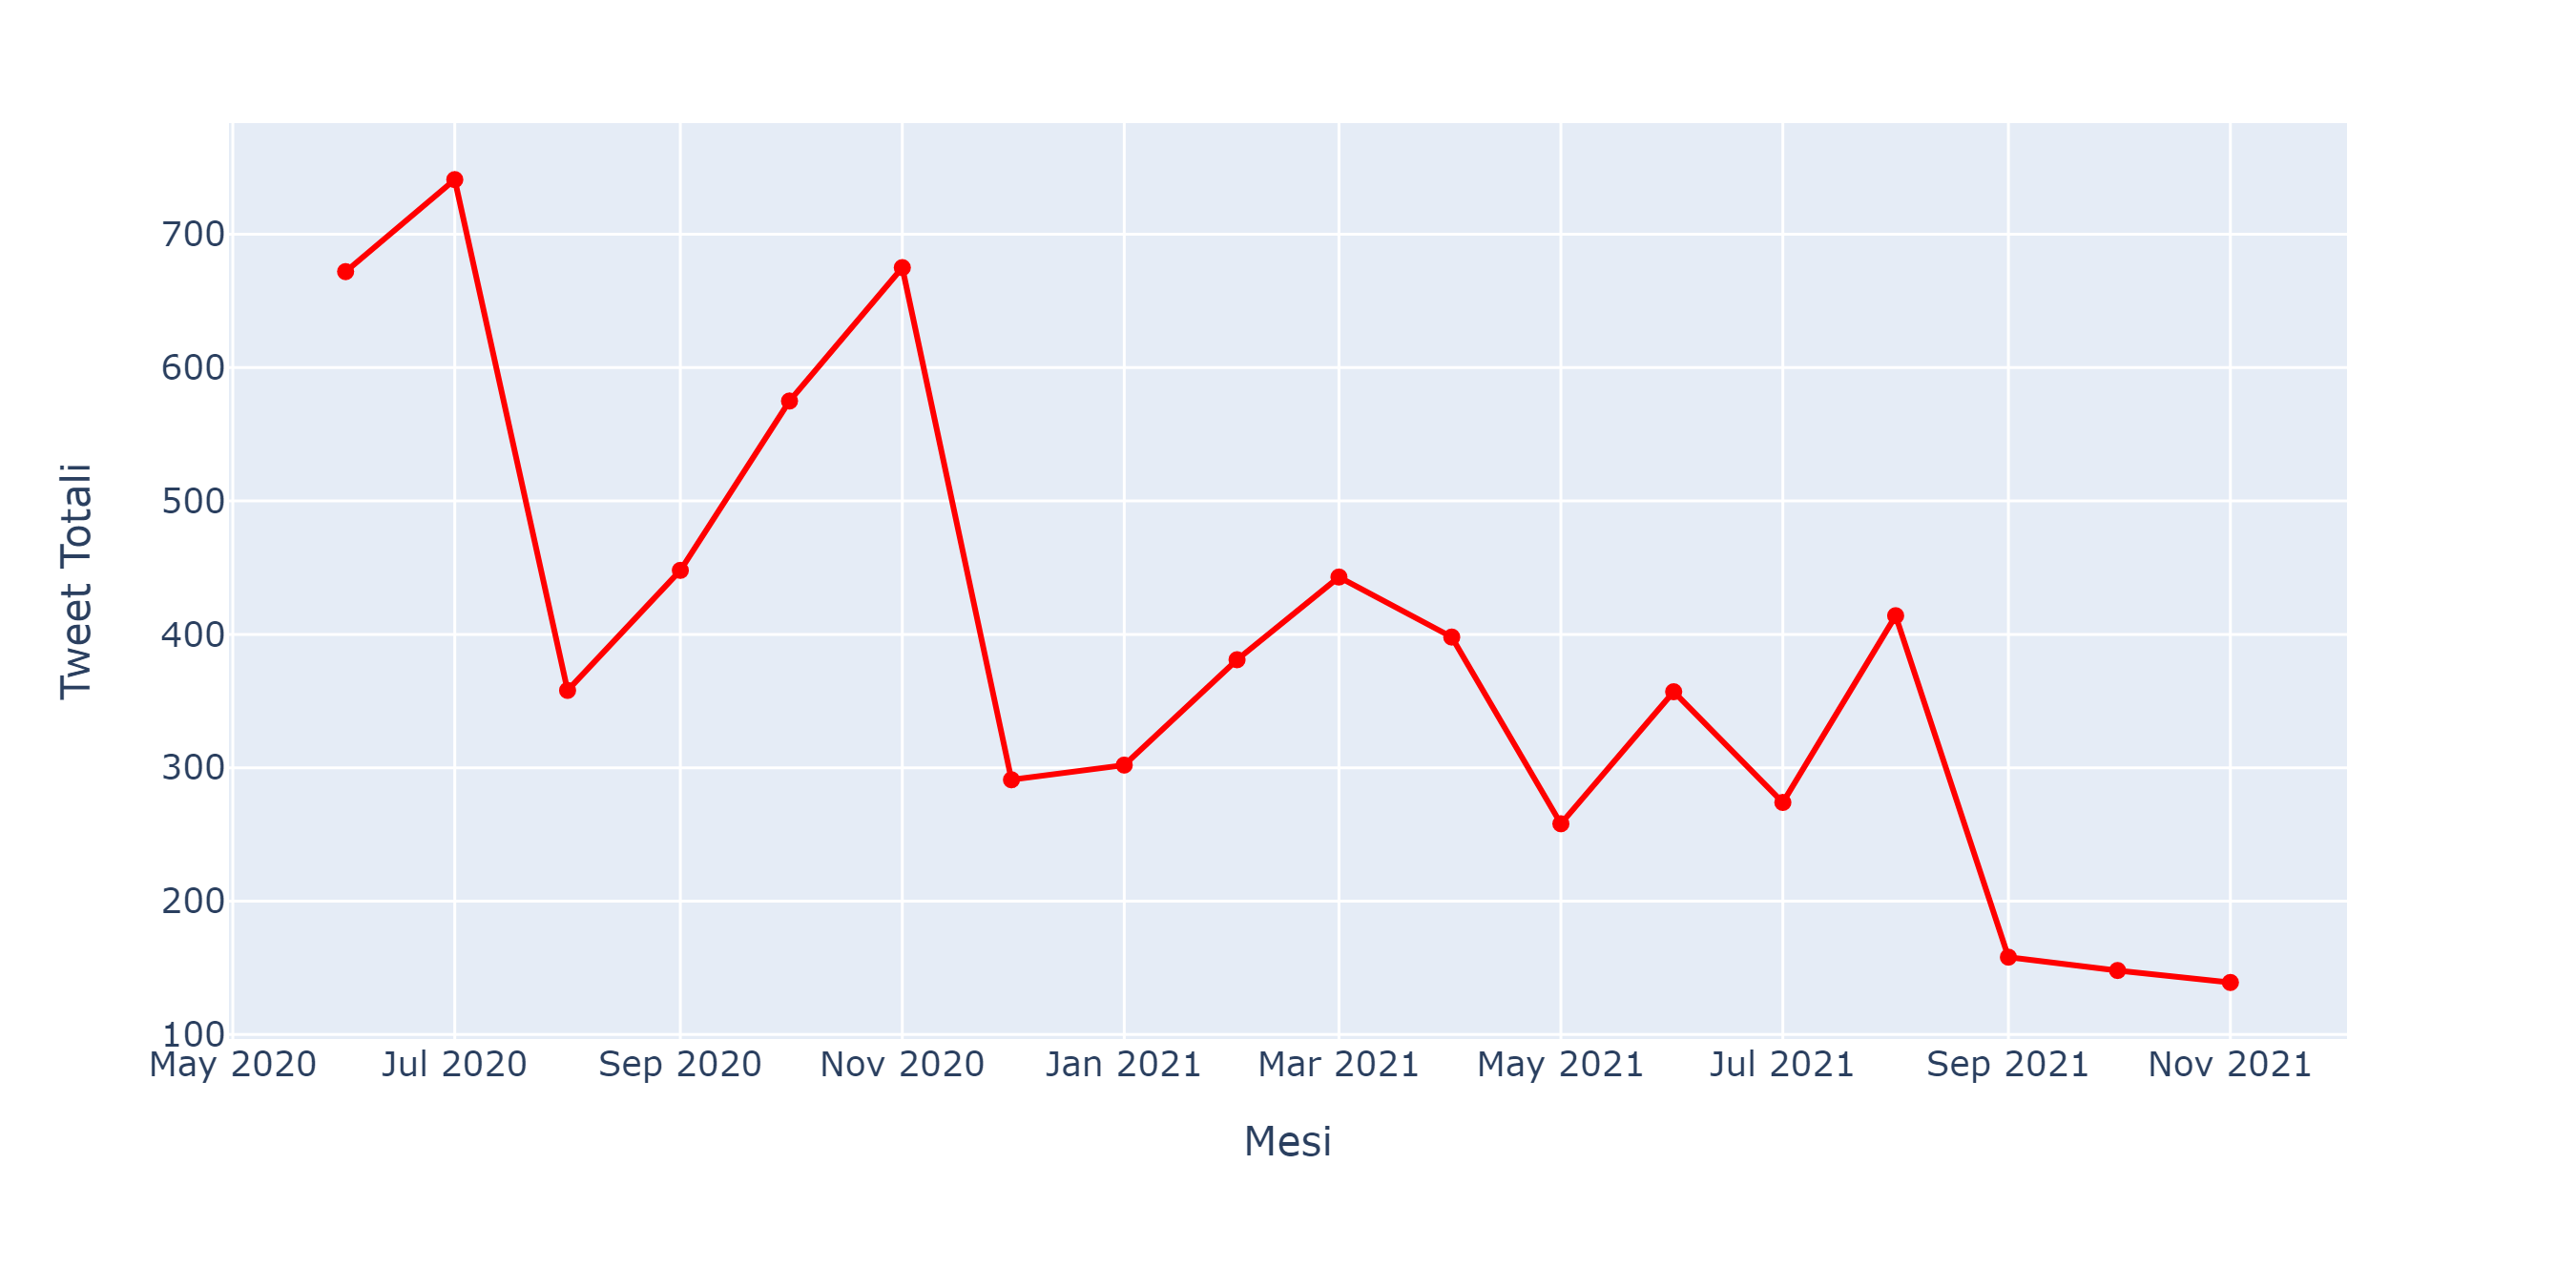
\includegraphics[width = 1\textwidth]{img/tweet_mesi.png}
    \caption{Andamento temporale dei tweet pubblicati sull'app Immuni tra giugno 2020 e dicembre 2021}
    \label{fig:tweet_mesi}
\end{figure}
Come si può vedere dal grafico in figura \ref{fig:tweet_mesi} ci sono stati alcuni periodi in cui c'è stato un maggiore dibattito tra gli utenti sul tema app Immuni, come quello avvenuto tra giugno e luglio 2020, mesi in cui per la prima volta l'applicazione viene rilasciata a livello nazionale su tutti gli store digitali e in cui sono stati scritti in totale 1414 tweet (672 a giugno e 741 a luglio), per poi riprendere a ottobre e novembre 2020, mesi in cui i contagi sono aumentati esponenzialmente dopo il calo durante i mesi estivi, con circa 600mila casi al giorno\footnote{Fonte: Monitoraggio situazione Covid-19 della Protezione Civile, disponibile all'indirizzo: \url{https://mappe.protezionecivile.gov.it/it/mappe-emergenze/mappe-coronavirus/situazione-desktop}}, fenomeno che ha portato gli utenti a discutere nuovamente sul tema e sulla sua efficacia nel monitoraggio dei casi. %Inoltre, in quel periodo, sono state stanziate le cosiddette "zone", dove in base al numero di contagi registrati in una regione ad essa veniva assegnato un colore (rosso, giallo, bianco) che rappresentavano un maggiore numero di restrizioni per la popolazione in termini di spostamenti dentro e fuori dalla regione e accesso ai luoghi pubblici.  % da rivedere
In questi mesi il totale dei tweet scritti sul tema è leggermente inferiore a quelli scritti a giugno e luglio (1250 tweet in totale).

A partire dal 2021, invece, la discussione sull'app Immuni comincia a diminuire con una media di 300 tweet al mese, per poi calare nei mesi finali, con un media di circa 150 tweet scritti nei mesi di settembre, ottobre e novembre 2021, un numero molto inferiore rispetto a quelli dell'anno precedente. Questo dato è probabilmente dovuto alla scarsa promozione dell'applicazione da parte delle cariche istituzionali, ma anche dalla riduzione delle misure restrittive grazie all'inizio della campagna vaccinale.

Tuttavia, ad agosto 2021 si registra un leggero aumento dei tweet sul tema (414 tweet), forse dovuto all'introduzione come stabilito dal Decreto Legge n 105 del 23/07/2021\footnote{D.L. n 105 23/07/2021, consultabile sulla Gazzetta Ufficiale all'indirizzo: \url{https://www.gazzettaufficiale.it/eli/id/2021/07/23/21G00117/sg})} della Certificazione Verde o \textit{Green Pass}, uno strumento scaricabile sul sito del Governo, che veniva assegnato ai cittadini guariti da Covid o che avevano ricevuto una o due dosi di vaccino che permette di accedere a molti servizi pubblici come scuole, luoghi di intrattenimento e strutture sanitarie. 
Questo fenomeno è in qualche modo collegato all'app Immuni, in quanto in quel periodo all'interno dell'applicazione è stata implementata la funzione di poter contenere il Green Pass in modo tale da facilitarne la reperibilità da parte dei cittadini. 
Tuttavia, questa nuova funzione sembra non aver risolto i problemi e lo scarso successo dell'applicazione che infatti nei mesi successivi è tornata ad essere inutilizzata.









\chapter{Metodologia}
Di seguito, una breve panoramica delle tecnologie automatiche e semi-automatiche utilizzate per analizzare i tweet raccolti nelle fasi successive ed estrarre informazioni utili per lo scopo della nostra indagine.

\section{Analisi linguistica dei tweet}
Per analizzare i tweet raccolti dal punto di vista linguistico si utilizzerà la libreria \textbf{NLTK} (Natural Language ToolKit) per eseguire alcune operazioni linguistiche di base sui tweet come la \textbf{tokenizzazione}, ossia la divisione dei tweet in tokens le unità base dell'analisi linguistica e la \textbf{lemmatizzazione}, necessaria per trasformare ciascun token in un \textbf{lemma}, ossia la forma originaria che si trova come voce di un dizionario.
Su questi token verranno poi estratte alcune informazioni di base, come il numero complessivo, la lunghezza interna e la quantità di token presenti in ciascun tweet, ma anche informazioni più avanzate la loro distribuzione, individuando i token più frequenti.
%La PNL combina la linguistica computazionale - la modellazione del linguaggio umano basata su regole - con modelli statistici, di apprendimento automatico e di apprendimento profondo. Insieme, queste tecnologie consentono ai computer di elaborare il linguaggio umano sotto forma di testo o dati vocali e di "comprenderne" il significato completo, con l'intento e il sentimento di chi parla o scrive. che si occupa dello studio di una lingua dal punto di vista della "forma" tramite l'estrazione delle informazioni linguistiche necessarie per monitorare uno o più aspetti di una lingua a partire da un corpus annotato con diverse informazioni di natura linguistica.

%Ad oggi, il monitoraggio linguistico è diventato uno strumento molto importante e ampiamente utilizzato per lo studio delle caratteristiche di una lingua grazie all'implementazione di tecniche linguistico-computazionali di annotazione sempre più efficienti che operano sui vari livelli della struttura testuale.
%In particolare, oggi, grazie a queste tecniche di annotazione automatica del testo, è possibile studiare corpora sempre più grandi che in passato venivano annotati con tecniche manuali o semi-automatiche (\cite{montemagni_tecnologie_2013}) ed estrarre informazioni utili per analisi successive.
%Nello specifico, per analizzare il nostro corpus, composto dai tweet scritti sul tema App Immuni la cui costruzione è stata descritta nel capitolo precedente, si seguirà la cosiddetta \textit{Pipeline} di annotazione linguistica, ossia una catena di analisi formata da modelli di annotazione ordinati in senso crescente dove ad ogni livello di annotazione viene aggiunto un nuovo tipo di informazione testuale. \\

\section{Analisi dei sentimenti e dei temi:  \textit{Sentiment Analysis} e \textit{Topic Modeling} }
Dopo aver analizzato i tweet dal punto di vista strettamente linguistico, verranno poi eseguite due operazioni molto utili per estrarre informazioni riguardanti sia le opinioni, le emozioni e le credenze degli utenti che i temi più discussi, con l'utilizzo di due tecniche: la \textit{Sentiment analysis} e il \textit{Topic Modeling}

\subsection{Sentiment Analysis} \label{sec: sent_an}
Le \textbf{emozioni} sono un elemento molto importante nelle discussioni tra gli individui, soprattutto quelle in abito politico e nel marketing, in cui esse vengono utilizzate frequentemente nelle pubblicità per suscitare un interesse verso il prodotto da vendere. \\
Tuttavia, recentemente le emozioni hanno un ruolo sempre più importante anche nelle discussioni che avvengono sul web, in quanto gli utenti scrivono spesso post o commenti con un tono che può essere collegato ad un'emozione o ad una combinazione di emozioni.

Esistono quindi molte tecniche automatiche che permettono di estrarre le emozioni degli autori a partire da una risorsa testuale come la tecnica di Natual Language processing che prende il nome \textbf{Sentiment Analysis}.

Il \textit{Natural Language Processing - NLP} è una branchia dell'informatica, e più precisamente dell'intelligenza artificiale, che si occupa di dare ai computer la capacità di comprendere testi e parole pronunciate in modo simile a quello degli esseri umani, combinando la linguistica computazionale (ossia la modellazione del linguaggio tramite l'utilizzo di regole) con modelli statistici di apprendimento automatico, o \textit{Machine Learning} e apprendimento profondo, o \textit{Deep Learning} in modo tale da far comprendere al computer il linguaggio umano rendendolo così capace di comprendere testi, di emulare il linguaggio umano e addirittura comprendere il significato e il contesto di un particolare linguaggio scritto o orale.
Queste tecniche sono attualmente molto utilizzate in vari ambiti e sono alla base di molti sistemi di utilizzo quotidiano, come i traduttori automatici e gli assistenti vocali. 

La \textbf{Sentiment Analysis} è dunque una tecnica di Natural Language Processing (NLP), utilizzata per estrarre, a partire da grandi quantità di dati, il pensiero, l'atteggiamento, i punti di vista, le opinioni, le credenze, i commenti, le richieste, le domande e le preferenze espresse da un autore sulla base di un'emozione espressa sotto forma testuale, nei confronti di entità come servizi, questioni, individui, prodotti, eventi, argomenti e organizzazioni (\cite{lamba_sentiment_2022}).
Questa tecnica viene spesso utilizzata nell'ambito del web per rilevare le emozioni degli utenti sul web e di conseguenza comprendere la loro posizione riguardo ad un particolare argomento che ha creato dibattito tra gli utenti.

Infatti, in questa relazione, la suddetta tecnica verrà utilizzate per estrarre, a partire dai tweet scritti dagli utenti, le loro emozioni e nei confronti dell'app Immuni, cercando di capire quali siano le emozioni più diffuse e la loro tipologia, ossia se esiste una \textit{polarizzazione} degli utenti verso un sentimento negativo, positivo o neurale nei confronti dell'applicazione.
Per fare ciò utilizzeremo un particolare tipo di Sentiment Analysis, il modello \textbf{\textit{Feel-It}}\footnote{la cui documentazione è disponibile al seguente repository GitHub:\url{https://github.com/MilaNLProc/feel-it}} sviluppato nel 2021 dal MilanNLP Lab\footnote{https://milanlproc.github.io/}, il laboratorio di Natural Languge Processing dell'Università Bocconi di Milano, per eseguire la Sentiment Analysis su testi scritti in lingua italiana, il quale si basa sulla creazione di un corpus in italiano annotato secondo quattro emozioni: "\textit{gioia}", "\textit{paura}" "\textit{tristezza}" e "\textit{rabbia}" (\cite{bianchi_feel-it_2021}).
La scelta di questo modello è giustificata dal fatto che i tweet scritti sul tema App Immuni sono scritti in lingua italiana e l'utilizzo di questo modello avrebbe portato a risultati più accurati rispetto ad altri utilizzati invece per estrarre emozioni a partire da altre lingue, come quello elaborato per la lingua inglese da \cite{abdul-mageed-ungar-2017-emonet}.


 
\subsection{Topic Modeling} \label{sec:TopicModeling}
L'operazione di \textbf{Topic Modeling} o identificazione degli argomenti, è una tecnica di elaborazione automatica del testo impiegata per l'estrazione degli argomenti presenti all'interno di risorse testuali, raggruppandoli all'interno di \textit{clusters} o gruppi di argomenti.

Tuttavia, molte delle tecniche convenzionali, come la Latent Dirichlet Allocation (LDA) (Blei et al., 2003) non risultano ottimali per l'analisi linguistica perché non tengono conto un fattore molto importante, ossia il contesto in cui le parole sono inserite all'interno della stessa frase, descrivendo il documento come un insieme di parole scollegate tra di loro.
Per questo motivo, negli ultimi anni sono state sviluppate diverse tecniche di \textit{embedding} come il Bidirectional Encoder Representations from Transformers (BERT) (\cite{devlin-etal-2019-bert}) e le sue varianti (ad esempio, si veda quanto riportato in \cite{lee_bioinformatics_2019}), che hanno mostrato grandi risultati poiché codificano le parole e le frasi come vettori e li raggruppano in base alla loro similarità nello spazio vettoriale. Queste tecniche vengono sia utilizzate dai motori di ricerca, sia per estrarre e clusterizzare gli argomenti dei testi come dimostrato da \cite{sia-etal-2020-tired} secondo cui una parola può fare parte di un argomento o topic e quindi di un cluster se essa è molto frequente in qual particolare cluster.

Per condurre la nostra analisi verrà utilizzata una particolare tecnica di Topic Embedding derivata dall'orginale BERT, ossia il \textbf{BERTopic},  il quale estrae gli argomenti seguendo tre fasi.
Come prima cosa, ogni documento presente all'interno del corpus in analisi viene convertito in embedding, ossia in un vettore, utilizzando un modello linguistico pre-addestrato.
Successivamente vengono ridotte le dimensioni di questi embedding al fine di ottimizzare il processo di clusterizzazione. Infine, a partire da questi cluster vengono estratti gli argomenti più frequenti all'interno dei documenti e ordinati in ordine di frequenza all'interno del corpus.

Il BERTopic verrà utilizzato nell'ultima fase del lavoro per estrarre i temi più frequenti che ricorrono nei tweet scritti sul tema app Immuni, i quali verranno utilizzati per analizzare possibili correlazioni o gerarchizzazioni tra gli argomenti.


\chapter{Risultati dell'analisi linguistica}

\section{Informazioni linguistiche di base}
Dopo aver compreso la natura dei nostri dati e aver eliminato valori nulli o non utili, concentrandosi sui tweet e analizzando i loro aspetti linguistici cercando di estrarre informazioni utili, utilizzando la libreria NLTK - Natural Language ToolKit\footnote{http://www.nltk.org}


% Prima di poter effettuare queste operazioni è stato necessario ripulire i tweet da eventuali elementi (spazi doppi, punteggiatura, lettere maiuscole, links ecc.) e simboli non utili ("@" e "\#" che precedono le menzioni e gli hashtag) , utilizzando le \textbr{espressioni regolari/Regular expression} e dalle cosiddette \textit{stopwords}, ossia tutte quelle parole che pur essendo molto comuni all'interno della lingua non sono funzionali al fine delle analisi linguistiche e non vengono indicizzate dai motori di ricerca (es. articoli, congiunzioni, preposizioni, ecc.)\\

Ciascun tweet è stato poi diviso in \textbf{tokens}, i quali sono stati successivamente \textit{lemmatizzati}, ossia riportati alla loro forma originaria \\
I token totali estratti dal corpus sono 146921 e in media ciascun tweet contiene circa 15 tokens (figura \ref{lunghezza_tok_tweet}); per quanto riguarda invece la lunghezza media dei tweet, ossia da quante lettere è composto ciascun token, la maggior parte dei token ha una lunghezza di 10 lettere (Figura \ref{Lunghezza_tok})

\begin{figure}[H]
	\centering
	\subfloat[]
	{
		\label{lunghezza_tok_tweet}
		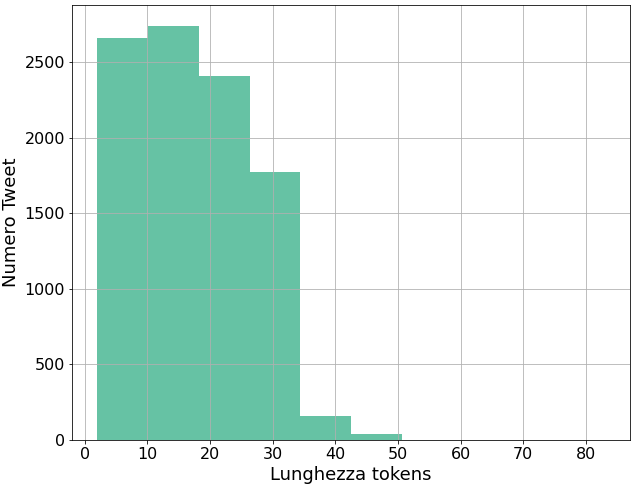
\includegraphics[width=.46\textwidth]{img/lunghezza_media_tokens_unici.png}
	}
	\quad
	\subfloat[]
	{
		\label{Lunghezza_tok}
		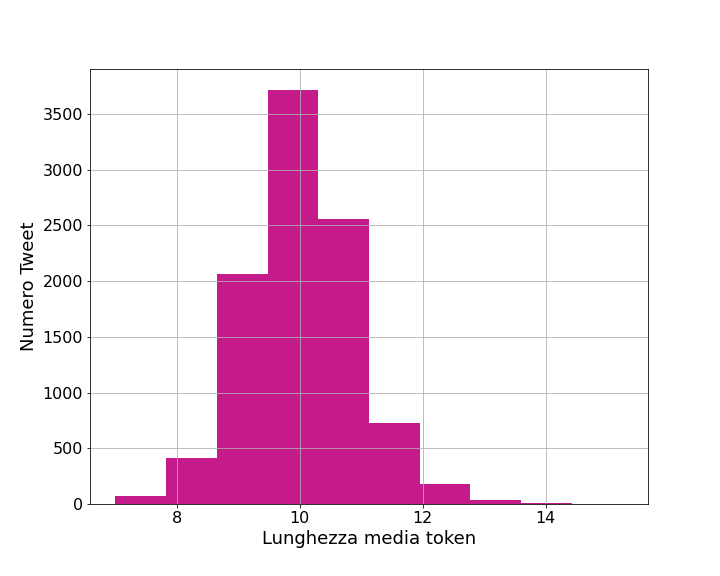
\includegraphics[width=.46\textwidth]{img/lunghezza_media_tokens.png}
	}    
	\setlength{\belowcaptionskip}{-10pt}
	\caption{Quantità media di tokens contenuti in ciascun tweet e lunghezza media dei tokens}
	\label{fig: tokens}
\end{figure}

\section{Analisi delle parole più frequenti}
Successivamente, si è provveduto ad analizzare quali fossero le parole più frequenti all'interno dei tweet, calcolando per ciascuna la propria frequenza all'interno del corpus.
\begin{figure} [H]
    \centering
    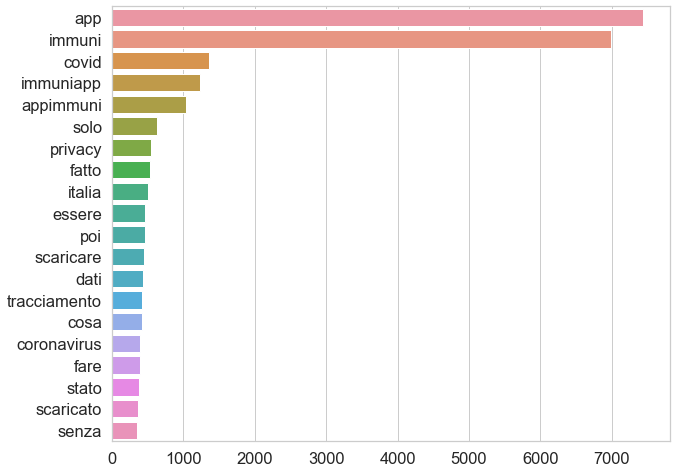
\includegraphics[width = 0.8\textwidth]{img/freq_toj.jpg}
    \caption{20 parole più utilizzate dagli utenti per discutere del tema App Immuni}
    \label{fig:most_common_20_tok}
\end{figure}
Analizzando le 20 parole più utilizzate all'interno dei tweet (figura \ref{fig:most_common_20_tok}), è possibile notare come tutte siano collegate al tema App Immuni e in generale al macro tema Coronavirus. Oltre a queste, altre due parole molto utilizzate sono \textit{dati}, che compare 436 volte nei tweet, e \textit{privacy} che compare 548 volte. Queste due parole sono molto importanti nella discussione sul tema App Immuni, in quanto spesso gli utenti sono molto restii a cedere i propri dati, soprattutto di natura sanitaria o di geo localizzazione, ad una applicazione di proprietà istituzionale, nonostante questi vengono ceduti ad altre piattaforme come ad esempio quelle dei maggiori \textit{social networks.}


Questa reticenza nella cessione dei dati è forse sintomo di una scarsa informazione da parte degli organi istituzionali, un fenomeno che ha poi portato al calo dei download di Immuni e al suo progressivo inutilizzo.


\section{Analisi degli \textit{hashtag} utilizzati}
Un altro aspetto che si è scelto di analizzare in questa fase del lavoro sono gli \textbf{hashtag} utilizzati dagli utenti per esprimersi sul tema App Immuni.
Gli hashtag sono uno strumento molto utilizzato su Twitter in quanto permettono di raggruppare tutti i tweet scritti su un particolare tema, facilitando all'utente la loro reperibilità; è sufficiente, infatti, che l'utente clicchi su quel particolare hashtag per risalire a tutti i tweet scritti sul tema.
% analisi hashtag
\begin{figure} [H]
    \centering
    
    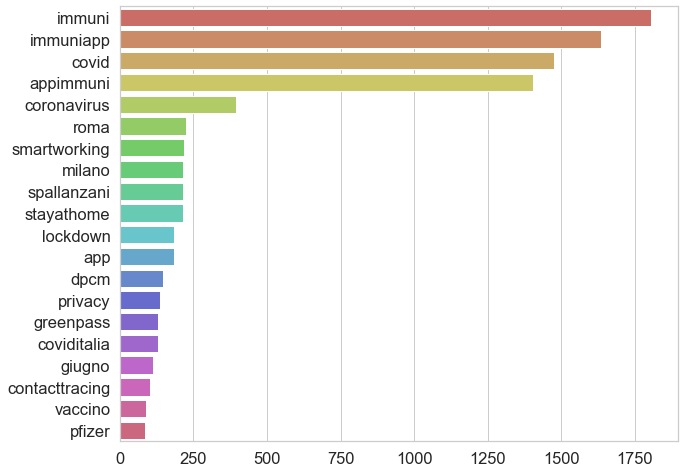
\includegraphics[width = 0.8
    \textwidth]{img/hash_most_freq.jpg}
    \caption{20 hashtag più utilizzati dagli utenti per discutere del tema App Immuni}
    \label{fig:hasht_tweet}
\end{figure}

Il grafico in figura \ref{fig:hasht_tweet}, mostra i dieci hashtag più utilizzati all'interno dei tweet, i quali sono per maggior parte correlati al tema App Immuni e, in generale al Coronavirus, con termini come (\textit{\#covid, \#coronavirus \#smartworking \#lockdown \#dpcm}\footnote{Decreto del Presidente del Consiglio dei ministri, atto amministrativo provvisorio avente forza di legge emanato dal Presiedente del Consiglio sotto la propria responsabilità in casi straordinari di emergenza o necessità}). Oltre a questi hashtag compaiono anche due nomi di città, Roma e Milano, molto importanti soprattutto per i loro ospedali che fin dall'inizio della pandemia si sono impegnate nella ricerca di cure.


Così come si osservava nel grafico \ref{fig:most_common_20_tok}, il termine privacy, oltre ad essere un termine molto utilizzato nei tweet è anche uno degli hashtag utilizzati maggiormente, comparendo in 136 tweet, dimostrando come il tema della privacy abbia acceso il dibatttito diventando uno dei macrotemi di Immuni
Oltre a questo hashtag, un altro molto utilizzato è \textit{\#GreenPass} che compare in 129 tweet scritti nel 2021, un aspetto che conferma ciò che si era osservato nel grafico in figura\ref{fig:tweet_mesi}, in cui nell'agosto 2021 si era osservato un leggero aumento dei tweet dovuti all'integrazione del Green Pass all'interno di Immuni e l'obbligo vaccinale, un tema molto dibattuto e delicato che ha spesso accesso molte discussioni e polarizzato gli utenti. Per questo motivo in alcuni tweet in cui si discute dell'App Immuni vengono quindi utilizzati hashtag come \#\textit{vaccino} e \#\textit{pzfer} che compaiono in circa 80 tweet.


Analizzando invece le caratteristiche linguistiche interne agli hashtag e, in particolare, la lunghezza interna degli hashtag, ossia quante sono le parole che li compongono, si nota come la maggior parte di essi sono molto breve e in media essi sono composti da 6 lettere, un dato che non sorprende vista la brevità dei tweet in termini di caratteri e il fatto che gli hashtag più utilizzati come \#immuni e \#Covid19 hanno quella lunghezza lessicale (Figura \ref{fig: lungh_media_hash_tweet})  
\begin{figure}[H]
    \centering
    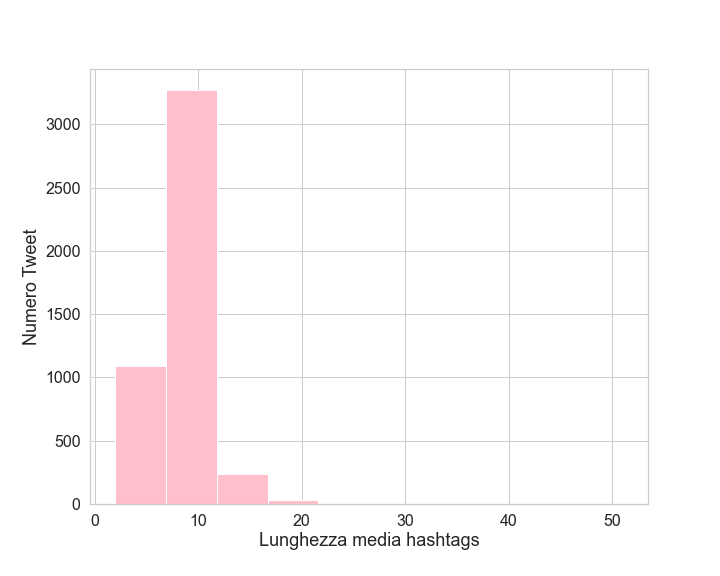
\includegraphics[width=.6
    \textwidth]{img/lunghezza_media_hasht_tweet.png}
    \caption{Quantità media degli hashtag contenuti in ciascun tweet e lunghezza media dei hashtag}
    \label{fig: lungh_media_hash_tweet}
\end{figure}

\section{Distribuzione di \textit{unigrammi}, \textit{bigrammi} e \textit{trigrammi}}
In ultima analisi si è scelto di analizzare la distribuzione delle parole più utilizzate dagli utenti e le combinazioni di parole più frequenti per discutere del tema in analisi.

Per quanto riguarda le singole parole, ossia gli unigrammi (figura \ref{unigrammi}), anche in questo caso abbiamo ottenuto risultati simili a quelli visti precedentemente. Infatti, come si può vedere dalle figure le quali rappresentano rispettivamente la distribuzione degli unigrammi, le parole più utilizzate riguardano il tema appImmuni.

Nel caso invece dei bigrammi (figura \ref{bigrammi}), combinazioni di due parole e dei trigrammi (Figura \ref{trigrammi}), combinazione di tre parole, più frequenti oltre al tema App Immuni, vengono utilizzate fa loro coppie e insiemi di parole rappresentativi della pandemia come \textit{Smartworking} e \textit{Spallanzani}, ossia uno degli ospedali più importanti e impegnati nella ricerca di cure contro il virus 
\begin{figure}[H]
	\centering
	\subfloat[]{
		\label{unigrammi}
		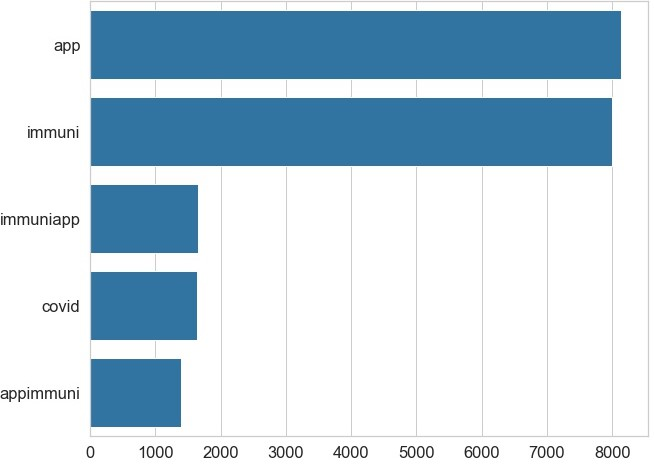
\includegraphics[width=.45\textwidth]{img/unigrammi_df_finale.jpg}
	}
	\quad
	\subfloat[]
	{
		\label{bigrammi}
		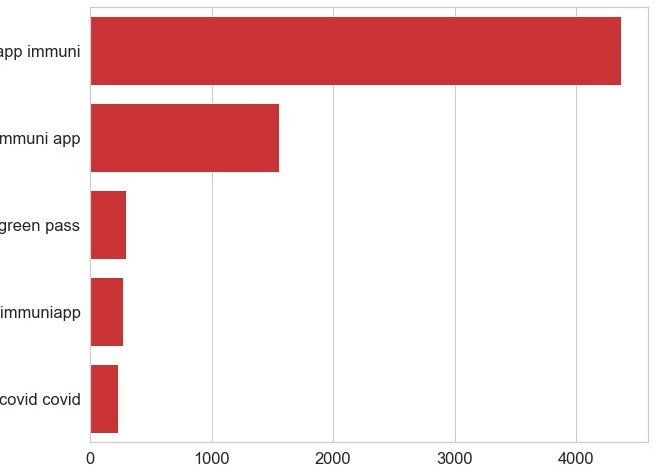
\includegraphics[width=.45\textwidth]{img/bigrammi_df_finale.jpg}
	}    
	\quad
	\subfloat[]
	{
		\label{trigrammi}
		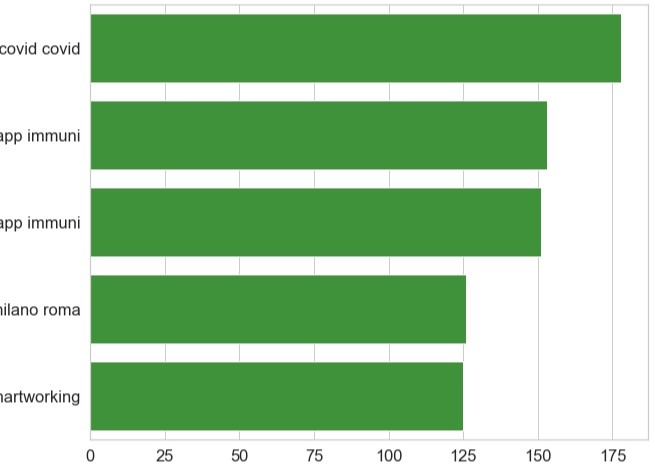
\includegraphics[width=.45\textwidth]{img/trigrammi_df_finale.jpg}
	}    
	\setlength{\belowcaptionskip}{-10pt}
	\caption{Distribuzione dei 5 unigrammi, bigrammi e trigrammi più frequenti utilizzati nella scrittura dei tweet}
	\label{fig: ngrams}
\end{figure}


\chapter{Risultati Sentiment Analysis con il modello \textit{Feel-It}}
L’ultima fase del lavoro riguarda l'analisi delle emozioni e dei temi più ricorrenti all'interno dei tweet scritti sul team app Immuni, in modo tale da comprendere meglio i problemi legati a questi app e gli aspetti su cui gli utenti discutono maggiormente.

Come illustrato in \ref{sec: sent_an}, per eseguire la Sentiment Analysis su questo corpus per classificare sia le emozioni che la tipologia di sentimenti, analizzando quindi la polarità, si utilizzerà il Modello \textit{Feel-It}

In particolare, per questa indagine si è scelto di analizzare le emozioni a due livelli di granularità differenti, applicando prima il modello a tutto il corpus e successivamente ai tweet scritti in due diversi periodi temporali: quelli scritti nel 2020 (6397 tweet) e quelli scritti nel 2021 (3387 tweet),  poiché la raccolta dei dati è avvenuta in un periodo molto lungo, in modo tale da evidenziare eventuali cambiamenti riguardo alle emozioni provate dall'utente riguardo all'utilizzo di Immuni.

\section{Analisi della polarità}
Innanzitutto, si è provveduto all'analisi della \textbf{polarità}, utilizzando il modello predittivo \textit{sentiment\_classifierier}, il quale estrarre dai dati i sentimenti, classificandoli in positivi e, negativi, applicandolo prima sull'intero insieme di tweet e successivamente sui due periodi temporali.
\begin{table}[H]
\centering
    \begin{tabular}{|l|c|c|c|}
    \hline
    \rowcolor[HTML]{DAE8FC} 
                       & \textbf{Tweet Totali} & \textbf{Tweet 2020} & \textbf{Tweet 2021} \\ \hline
    \textit{Negativi}    & 8580    & 5656  & 2924    \\ \hline
    \textit{Positivi}     & 1204   & 741   & 463                 \\ \hline
    \end{tabular}
    \caption{Risultato della classificazione effettuata dal Modello Feel-It sui tweet totali e di quelli scritti nel 2020 e 2021}
    \label{table: ris_fellit}
\end{table}
La tabella \ref{table: ris_fellit} mostra come in tutti e tre i corpora la maggior parte dei tweet siano negativi, sinonimo che in generale l'attitudine degli utenti nei confronti dell'App Immuni sia di natura negativa, un dato che giustificherebbe il progressivo fallimento dell'applicazione dovuto alla non coinvolgimento da parte degli utenti e in generale alla scarsa promozione dell'app da parte del Governo e alla crisi interna del Governo italiano che nel 2021 ha visto la caduta del Governo Conte avvenuta il 26 gennaio 2021 con le dimissioni di Giuseppe Conte e l'arrivo al potere del Presidente Mario Draghi, il quale però non si è ancora espresso sull'utilizzo dell'app.


\section{Analisi dei sentimenti}
Successivamente, si è scelto di analizzare le emozioni provate dagli utenti nel momento in cui pubblicano un tweet per esprimere la propria opinione sul tema App Immuni. Per eseguire questa indagine, è stato utilizzato un altro modello predittivo di Feel-It, il modello \textit{emotion\_classifier} che annota il corpus secondo 4 emozioni: paura, rabbia, gioia e tristezza. 
\begin{table}[H]
\centering
\begin{tabular}{|l|c|c|c|}
\hline
\rowcolor[HTML]{DAE8FC} 
                   & \textbf{Tweet totali} & \textbf{Tweet 2020} & \textbf{Tweet 2021} \\ \hline
\textit{Rabbia}    & 6249                  & 4021                & 2228                \\ \hline
\textit{Paura}     & 2507                  & 1779                & 728                 \\ \hline
\textit{Felicità}  & 721                   & 433                 & 288                 \\ \hline
\textit{Tristezza} & 307                   & 164                 & 143                 \\ \hline
\end{tabular}
\caption{Risultati della classificazione delle emozioni estratte dai tweet totali e da quelli pubblicati nel 2020 e 2021}
\label{tab: emotions}
\end{table}
I risultati derivati dall'applicazione di questo modello e illustrati nella tabella \ref{tab: emotions}, mostrano come le emozioni più rilevanti siano la rabbia e la paura, entrambe emozioni negative, che confermano quindi una polarità negativa degli utenti come si era visto precedentemente, e che in un certo senso sono legate al tema App Immuni, che ha spesso creato dibattito su temi riguardanti non solo la salute, ma anche la privacy e la cessione di dati sensibili, due aspetti che possono essere collegati al sentimento della paura e della rabbia da parte degli utenti. 
\begin{figure}[H]
	\centering
	\subfloat[]
	{
		\label{sent_an_2020}
		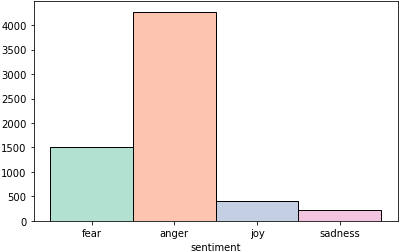
\includegraphics[width=.47\textwidth]{img/sentAnalysis2020.png}
	}
	\quad
	\subfloat[]
	{
		\label{sent_an_2021}
		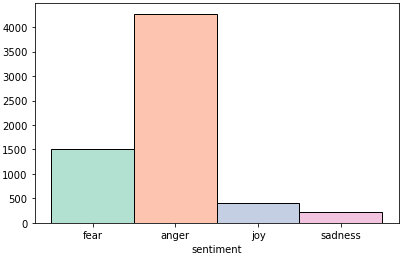
\includegraphics[width=.47\textwidth]{img/sentAnalysis2021.png}
	}    
	\quad
	\setlength{\belowcaptionskip}{-10pt}
	\caption{Distribuzione dei sentimenti all'interno dei tweet pubblicati nel 2020 (a destra), e nel 2021 (a sinistra)}
	\label{fig: sentan}
\end{figure}
Tuttavia, queste due emozioni si distribuiscono in maniera diversa all'interno dei due anni, diminuendo progressivamente nel 2021, un aspetto che può essere giustificato dal fatto i dati raccolti nel 2021 (Figura \ref{sent_an_2021}) sono minori rispetto a quelli del 2020  (Figura \ref{sent_an_2020}), fenomeno dovuto al fatto che con il passare del tempo l'app Immuni è andata pian piano in disuso per motivi sia politici, dovuti alla già citata mancata organizzazione e promozione, che sanitari grazie all'arrivo di misure di prevenzione più efficaci contro la diffusione del virus, come i vaccini.
Tuttavia, è possibile notare anche la presenza di una piccola percentuale di tweet classificati come \textit{gioia}, sintomo che alcuni utenti siano favorevoli all'utilizzo dell'applicazione, una percentuale che però non riesce a consolidare il successo dell'applicazione.

\begin{figure}[H]
	\centering
	\subfloat[]
	{
		\label{wordcloud_gioia}
		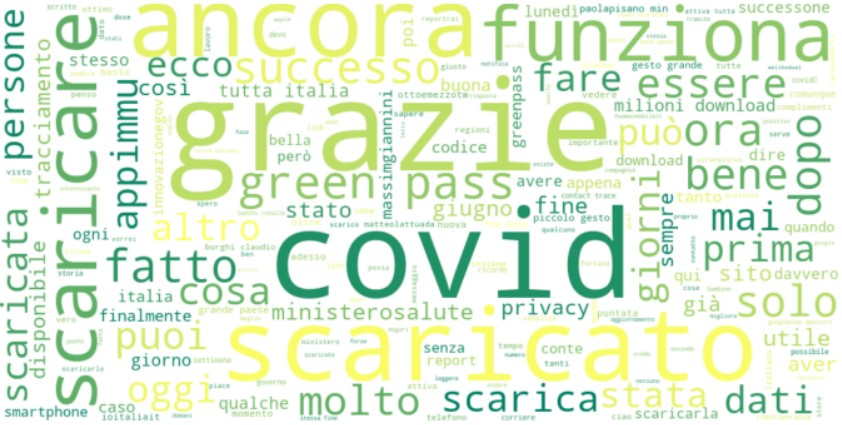
\includegraphics[width=.47\textwidth]{img/wordcloud_parole_gioia.jpg}
	}
	\quad
	\subfloat[]
	{
		\label{wordcloud_rabbia}
		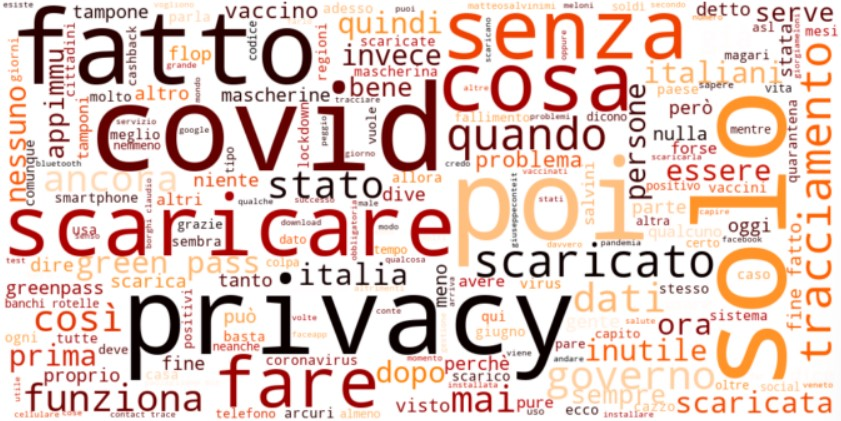
\includegraphics[width=.47\textwidth]{img/wordcloud_parole_rabbia.jpg}
	}    
	\quad
	\setlength{\belowcaptionskip}{-10pt}
	\caption{Parole più utilizzate nei tweet classificati come '\textit{goia}' (\ref{wordcloud_gioia}) e '\textit{rabbia}' (\ref{wordcloud_rabbia})}
	\label{fig: wordclouds}
\end{figure}

Infine, si è scelto di esaminare ulteriormente le emozioni estratte dai tweet, analizzando le parole più frequenti all'interno dei tweet classificate con le emozioni positive (corrispondenti alla gioia, Figura \ref{wordcloud_gioia}) e tra quelle negative quelle legate alla rabbia (Figura \ref{wordcloud_rabbia}).
Per semplificare l'analisi dei risultati si è scelto di rappresentare queste parole sotto forma di \textit{wordcloud}, una tecnica di rappresentazione visiva funzionale alla visualizzazione delle parole chiave più utilizzate grazie all'utilizzo di colori e dimensioni grafiche diverse che servono per identificare l'importanza di un termine all'interno di un insieme di parole. Nonostante nel caso della gioia tra le parole più ricorrenti compaiano 'grazie', 'funziona', nel caso della rabbia, che come si è visto è il sentimento prevalente all'interno del corpus, si evidenzia come la maggior parte degli utenti pubblichi tweet con argomenti legati soprattutto alla non fiducia nella campagna promozionale delle istituzioni nei confronti di Immuni, un fenomeno che potrebbe essere rappresentato dal termine "governo", e nel tracciamento eseguito utilizzando dati sensibili, un dato che viene giustificato dalla forte presenza di termini come \textit{privacy}, e \textit{dati} che come si è osservato anche nelle analisi precedente sono due dei termini che rappresentano i problemi maggiori legati a Immuni suscitando anche un forte dibattito tra gli utenti.

%In entrambi i casi le parole più frequenti, rappresentate utilizzando un \textit{font} più grande, sono tutte legate alle varianti del nome dell'applicazione (\textit{App, AppImmuni, ImmuniApp, Immuni}). 


\chapter{Analisi degli argomenti con BERTopic}

L'ultima analisi condotta in questa relazione riguarda l'identificazione dei temi più frequenti all'interno dei tweet, utilizzando la tecnica BERTopic, le cui caratteristiche sono state illustrate in \ref{sec:TopicModeling}.
Così come per la Sentiment Analysis, anche in questa ultima fase del lavoro si è scelto di analizzare il fenomeno sia in generale, ricercando i temi più ricorrenti in tutti i tweet, sia in un particolare periodo temporale che anche in questo caso corrisponde ai tweet pubblicati nel 2020 e nel 2021, così da poter notare se ci fosse un eventuale cambiamento nella distribuzione temporale degli argomenti.\\


Innanzitutto, prima di applicare il modello BERTopic ai dati, si è scelto di estrarre gli argomenti a partire dai tweet in cui sia presente un minimo di interazione tra gli utenti, considerando quindi tutti quelli con almeno un like e un retweet (1580 tweet), in modo tale da evitare di estrarre argomenti non rilevanti e allo stesso modo ridurre i tempi di esecuzione del processo. 

Successivamente, si è provveduto a creare per ciascun set di dati (tweet totali, tweet pubblicati nel 2020 e tweet pubblicati nel 2021) i vettori contenenti i tweet su cui verrà poi applicato il modello BERTopic per l'identificazione dei temi in lingua italiana.
Da questi vettori sono stati poi estratti per ciascun insieme di dati gli argomenti più frequenti, che in tutti i casi risultano molto correlati tra loro simili tra di loro, un dato che confermerebbe la forte correlazione tra i temi discussi dagli utenti in merito a Immuni.
\begin{figure} [H]
    \centering
    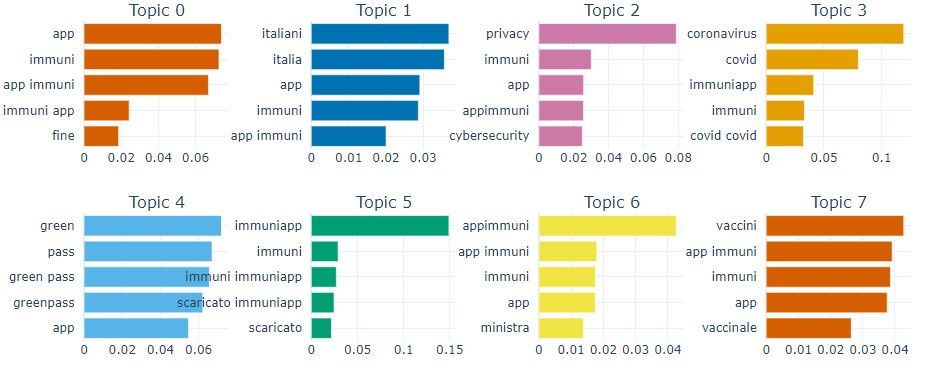
\includegraphics[width = 1\textwidth]{img/topics_tot.jpg}
    \caption{Argomenti più frequenti all'interno di tutti i tweet raccolti}
    \label{fig:topicMtot}
\end{figure}

Riguardo ai 10 temi estratti sul totale dei tweet (Figura \ref{fig:topicMtot}, è possibile notare come ci siano 3 diverse categorie di temi disposte secondo una gerarchia: quelli legati all'app in generale, quelli legati al green pass, alla privacy e alla sicurezza, tutti collegati al macro tema corrispondente al Topic 0 ossia il Coronavirus.

Analizzando invece i temi estratti dai tweet pubblicati nel 2020 e nel 2021 è possibile notare alcune differenze. 
\begin{figure}[H]
	\centering
	\subfloat[]
	{
		\label{topics_2020}
		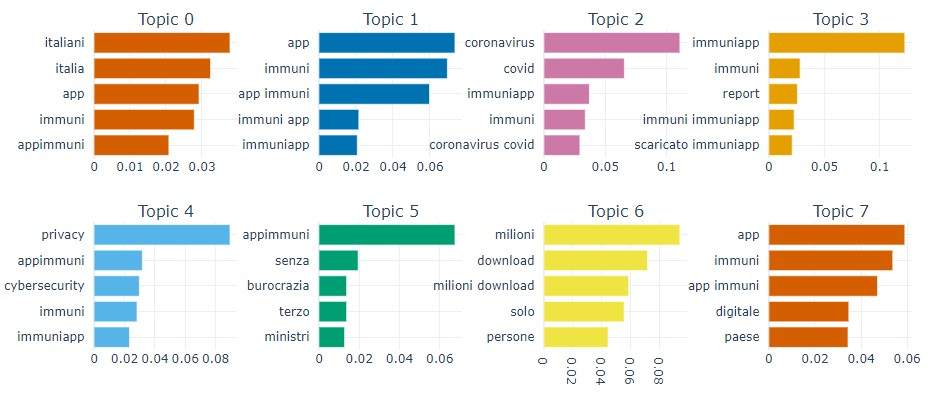
\includegraphics[width= 1\textwidth]{img/topics_2020.jpg}
	}
	\quad
	\subfloat[]
	{
		\label{topics_2021}
		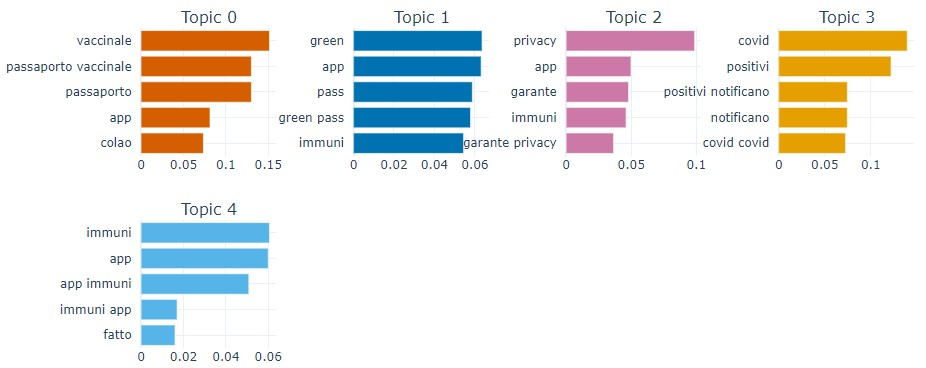
\includegraphics[width=1\textwidth]{img/topics_2021.jpg}
	}    
	\quad
	\setlength{\belowcaptionskip}{-10pt}
	\caption{Argomenti più ricorrenti nei tweet scritti nel 2020 (\ref{topics_2020}) e nel 2021 (\ref{topics_2021})}
	\label{fig: topicModels}
\end{figure}
La prima riguarda il numero di argomenti estratti, undici nel caso dei tweet scritti nel 2020 e sei nel caso di quelli scritti nel 2021, un aspetto che può essere giustificato dalle diverse dimensioni dei due insieme di dati (1107 tweet scritti nel 2020 e 473 nel 2021), mentre riguardo alla tipologia di temi individuati si nota come mentre nel 2020 (Figura \ref{topics_2020}) i temi più ricorrenti siano legati al Coronavirus e a Immuni, in cui emergono anche qui temi come la privacy, ma anche temi come i download e la burocrazia, nel 2021 (Figura \ref{topics_2021}), la discussione su Immuni è incentrata verso due temi molto influenti in quell'anno, ossia il Green Pass e la campagna vaccinale, rappresentati rispettivamente dal Topic 0 e Topic 1 in cui compaiono termini come appunto \textit{greenPass}, il quale viene indicato anche con il termine \textit{passaporto vaccinale}.

Da quest'ultima analisi emerge quindi nuovamente questa evoluzione dei temi trattati dagli utenti che dopo un iniziale interesse verso Immuni a causa dei forti contagi e della totale assenza di misure di prevenzione sufficientemente efficaci nel 2020, estendono nell'anno successivo la discussione sull'applicazione anche verso altri temi di tendenza come i vaccini e il Green Pass.
Tuttavia, il tema della privacy e della cessione dei dati continua ad essere un tema centrale in entrambi i periodi, sintomo che forse quello potrebbe essere uno dei problemi centrali che ha causato il graduale fallimento di Immuni.


\addcontentsline{toc}{chapter}{Conclusioni}
\input{conclusioni}

\addcontentsline{toc}{chapter}{Bibliografia}
\thispagestyle{empty}
\nocite{*}
\printbibliography

\addcontentsline{toc}{chapter}{Sitografia}
%\thispagestyle{empty}
%\nocite{*}
\chapter*{Sitografia }

Coronavirus. La situazione desktop. (s.d.). Recuperato 24 giugno 2022, da \url{https://mappe.protezionecivile.gov.it/it/mappe-emergenze/mappe-coronavirus/situazione-desktop}

Cos’è successo all’app Immuni. (2021, febbraio 18). Il Post.
\url{http://www.ilpost.it/2021/02/18/immuni-app-draghi/}

FEEL-IT: Emotion and Sentiment Classification for the Italian Language. (2022). MilaNLP. \url{https://github.com/MilaNLProc/feel-it}

Immuni—Sito Ufficiale. Recuperato 25 maggio 2022, da \url{https://www.immuni.italia.it/www.immuni.italia.it}

ItaliaNLP.. Recuperato 27 maggio 2022, da \url{http://www.italianlp.it/}
Matplotlib—Visualization with Python.Recuperato 27 maggio 2022, da \url{https://matplotlib.org/}

NLTK: Natural Language Toolkit. Recuperato 23 giugno 2022, da https://www.nltk.org/

Seaborn 0.11.2 documentation Recuperato 27 maggio 2022, da \url{https://seaborn.pydata.org/introduction.html}


TWINT Project. Recuperato 27 maggio 2022, da \url{https://github.com/twintproject}

\end{document}


